\documentclass{article}

\usepackage{arxiv}

\usepackage[utf8]{inputenc} % allow utf-8 input
\usepackage[T1]{fontenc}    % use 8-bit T1 fonts
\usepackage{hyperref}       % hyperlinks
\usepackage{url}            % simple URL typesetting
\usepackage{booktabs}       % professional-quality tables
\usepackage{amsfonts}       % blackboard math symbols
\usepackage{amsmath}
\usepackage{microtype}      % microtypography
\usepackage{graphicx}

\title{AI-assisted pharmaceutical analysis of prescriptions combining retrieval-augmented generation and a rule-based expert system}

% Authors in alphabetical order of last name
\author{
	Muhammad Awais \\
	INSERM UMR 1231 \\
	Dijon, France \\
	\texttt{awaisqadir923@gmail.com} \\
	\And
	Mathieu Boulin \\
	CHU Dijon Bourgogne \\
	Dijon, France \\
	\texttt{mathieu.boulin@chu-dijon.fr} \\
	\And
	Stéphanie Bricq \\
	ICube, CNRS \\
	Strasbourg, France \\
	\texttt{bricq@unistra.fr} \\
	\And
	Lucie Briottet \\
	CHU Dijon Bourgogne \\
	Dijon, France \\
	\texttt{lucie.briottet@outlook.fr} \\
	\And
	Davide Callegarin \\
	CHU Dijon Bourgogne \\
	Dijon, France \\
	% TODO: email not found
	\And
	Patrick Callier \\
	CHU Dijon Bourgogne \\
	Dijon, France \\
	\texttt{patrick.callier@chu-dijon.fr} \\
	\And
	Bastian Fouquier \\
	CHU Dijon Bourgogne \\
	Dijon, France \\
	\texttt{bastian.fouquier@chu-dijon.fr} \\
	\And
	Jessica Gobbo \\
	Centre Georges-François Leclerc \\
	INSERM UMR 1231 \\
	Dijon, France \\
	\texttt{jgobbo@cgfl.fr} \\
	\And
	Marie-Pierre Guenfoudi \\
	CHU Dijon Bourgogne \\
	Dijon, France \\
	\texttt{marie-pierre.guenfoudi@chu-dijon.fr} \\
	\And
	Isen Naiken \\
	CHU Dijon Bourgogne \\
	INSERM UMR 1231 \\
	ImVIA, Université Bourgogne Europe \\
	Dijon, France \\
	\texttt{isen.naiken@chu-dijon.fr} \\
	\And
	Mélodie Opale \\
	CHU Dijon Bourgogne \\
	Dijon, France \\
	% TODO: email not found
}

\renewcommand{\shorttitle}{AI-assisted pharmaceutical analysis of prescriptions}

\hypersetup{
pdftitle={AI-assisted pharmaceutical analysis of prescriptions combining retrieval-augmented generation and a rule-based expert system},
pdfsubject={cs.CL, cs.AI},
pdfauthor={Muhammad Awais, Mathieu Boulin, Stéphanie Bricq, Lucie Briottet, Davide Callegarin, Patrick Callier, Bastian Fouquier, Jessica Gobbo, Marie-Pierre Guenfoudi, Isen Naiken, Mélodie Opale},
pdfkeywords={Clinical pharmacy, Medication review, Large language model, Retrieval-augmented generation, Expert system},
}

\begin{document}
\maketitle

\begin{abstract}
	\textbf{Background.} % TODO

	\textbf{Methods.} We developed a pipeline that analyses each prescription in three steps. First, a retrieval module searches clinical guidelines for passages relevant to the patient. The guidelines are split into passages and stored in a vector database. One query is built for each prescription line, using the drug, its dose, its dosage regimen and the patient profile, including the renal function and abnormal laboratory values. The language model also writes short context sentences about the patient, which are used as additional queries. Second, a rule-based expert system, built on the CLIPS inference engine, checks the prescription against drug interaction rules, hospital-specific rules and statistical rules drawn from past pharmaceutical interventions, and returns alerts. New hospital rules are drafted by the language model from a request written in natural language and are saved only after the pharmacist has checked them. Third, a large language model receives the patient record, the alerts and the retrieved passages. It returns a structured opinion made of one to four points. Each point is an intervention, a verification, a monitoring or a validation, with the sources it relies on. The decision for the patient is the most severe point. A graphical interface allows pharmacists to run the analysis, read the results, open the cited sources, score the opinions, add documents and add new rules.

	\textbf{Results.} % TODO

	\textbf{Conclusion.} % TODO
\end{abstract}

\keywords{Clinical pharmacy \and Medication review \and Large language model \and Retrieval-augmented generation \and Expert system}


% TODO: Introduction

\section{Introduction}


\section{Methods}
\label{sec:methods}

\subsection{Overview}

The system analyses the prescription of each patient and returns a pharmaceutical opinion. It combines three modules: a retrieval module, a rule-based expert system and a large language model (LLM) (Figure~\ref{fig:architecture}). Before any analysis, the clinical guidelines are indexed in a vector database. For each patient, the retrieval module and the expert system are run first. Their outputs are then passed to the LLM, which gives the final decision. Separately from the analysis, pharmacists can add hospital-specific rules to the expert system with the help of the LLM.

Each patient record is stored in JSON format. It contains the patient identifier, a reference date and, when known, the age, weight, height, body mass index and body surface area. It also contains the most recent result of each laboratory test before the reference date, with its unit and date. Finally, it contains the prescription lines active on the reference date. Each line gives the drug label (product, strength and pharmaceutical form), the active ingredients with their dosage, the daily quantity and intake unit, a readable dosage regimen, the start and end dates, and whether the drug is given as needed.

\begin{figure}[ht]
	\centering
	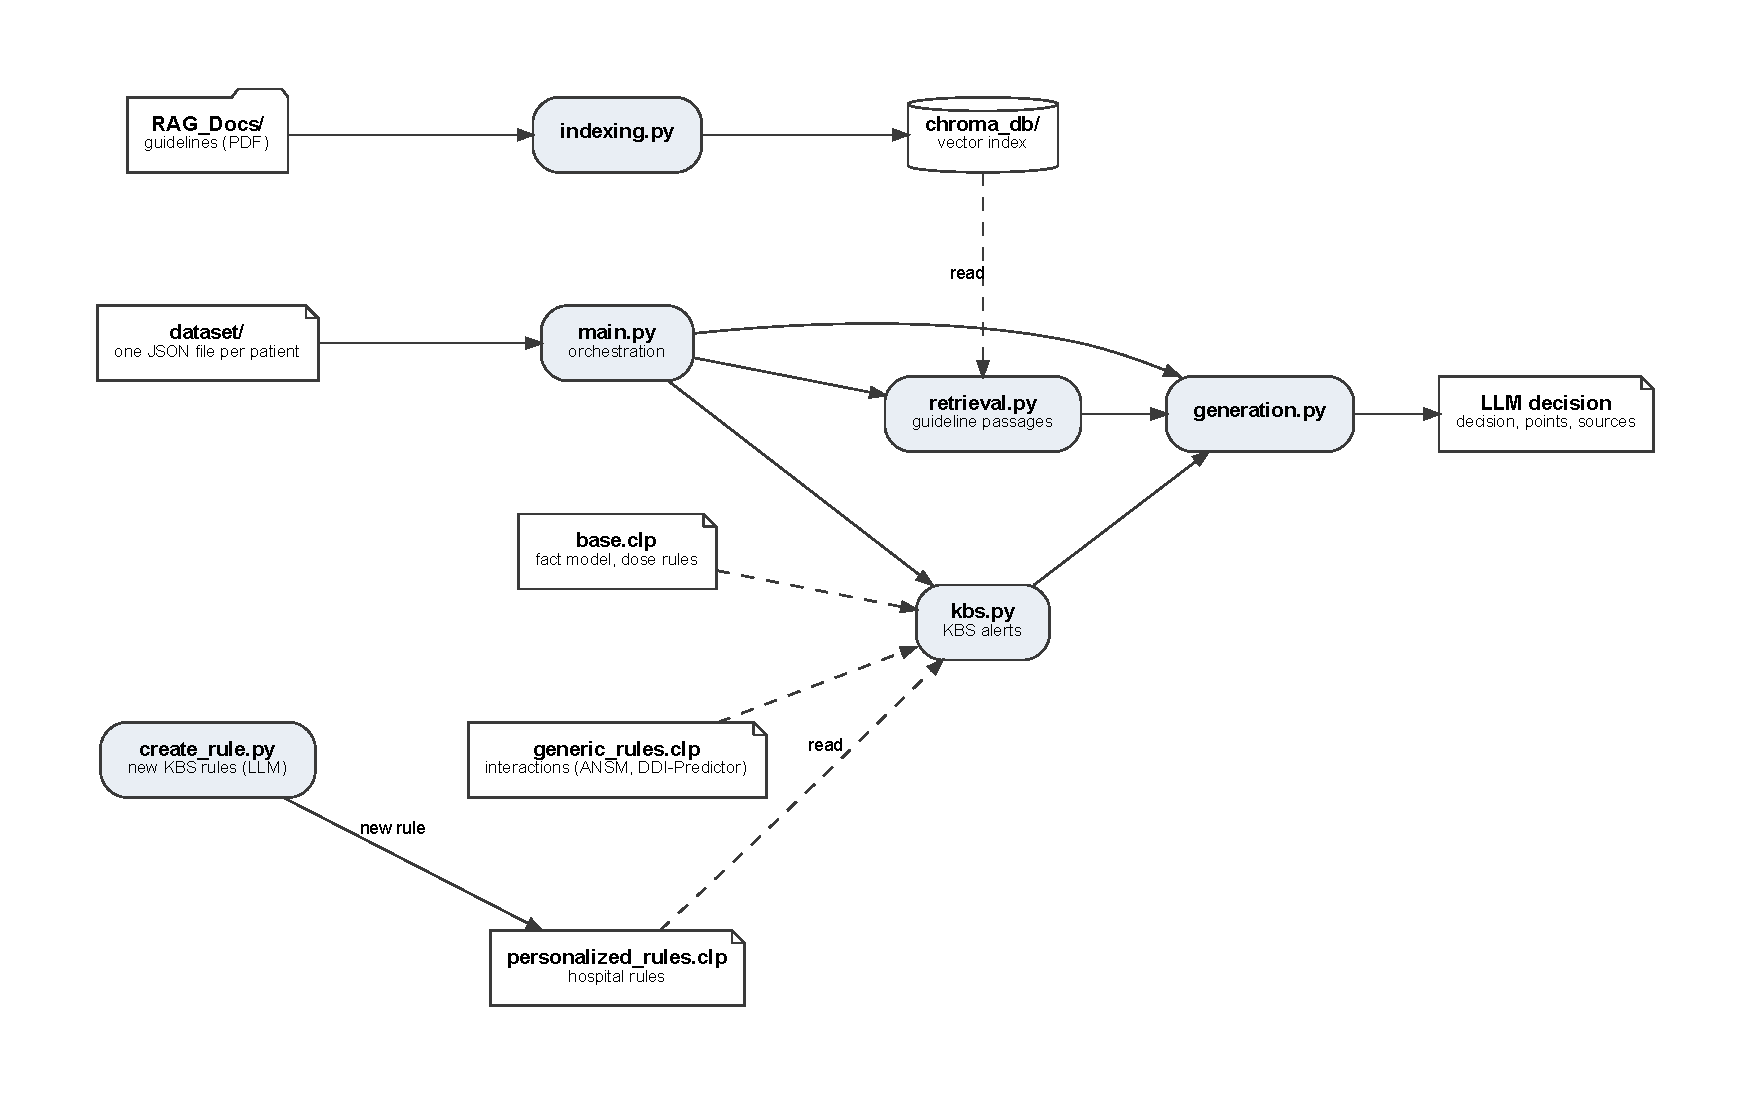
\includegraphics[width=\textwidth]{figures_en/figure_1.pdf}
	\caption{Overall architecture of the pipeline. Guidelines (PDF) are split into passages and indexed in a vector database (ChromaDB). For each patient, the retrieval module extracts relevant passages and the expert system (kbs.py) produces deterministic alerts. The expert system reads four rule files: the fact model and dose rules (base.clp), the drug interactions (generic\_rules.clp), the hospital rules (personalized\_rules.clp) and the statistical rules drawn from past pharmaceutical interventions (statistical\_rules.clp). New hospital rules are drafted by the language model (create\_rule.py) and saved in personalized\_rules.clp. The alerts and the passages are passed to the language model, which gives the final decision.}
	\label{fig:architecture}
\end{figure}

\subsection{Guideline indexing}

The document base contains clinical guidelines in PDF format. The current version includes four documents: the position statement of the French-speaking Diabetes Society (Société Francophone du Diabète, SFD) on the management of type 2 diabetes, and guidelines on urinary tract infections (SPILF), on heart failure and on the management after myocardial infarction. % TODO: add the full references of the four documents
Each PDF is converted to text page by page with PyMuPDF4LLM, without optical character recognition. The text of each page is split into passages of 1,500 characters, with an overlap of 200 characters between consecutive passages. Each passage keeps the name of its source file and its page number. Passages are encoded with the Qwen3-Embedding-8B model and stored in a ChromaDB database, using the cosine distance. New documents can be added at any time; they are indexed in the same way.

\subsection{Retrieval of relevant passages}

The retrieval module selects the guideline passages that are useful for a given patient (Figure~\ref{fig:retrieval}). It works in five steps.

\textbf{Clinical profile.} The renal function changes the dose of many drugs. The renal values (estimated glomerular filtration rate with the CKD-EPI equation, creatinine clearance with the Cockcroft-Gault equation and serum creatinine) are therefore always added to the profile when they are present, even when they are normal. Each other laboratory value is compared with a reference range defined by the pharmacists (for example, 4--6\% for HbA1c). Values outside the range are converted into short text descriptions, such as ``high HbA1c''. The renal values and these descriptions form a short clinical profile that also contains the age and weight of the patient.

\textbf{Search for each prescription line.} One query is built for each prescription line. It contains the drug name, dose, unit, dosage regimen and clinical profile. All queries are encoded with the same embedding model as the passages, preceded by a short task instruction, as recommended for this model. For each query, the three closest passages are retrieved from the database.

\textbf{Merging of results.} The same passage can be found by several queries. Duplicates are removed, and the smallest distance is kept for each passage. Passages are then sorted by distance, and the eight closest are kept.

\textbf{Context written by the LLM.} The queries of the second step describe the drug, its dose and the patient profile, but not the likely indication of the drug or the situation of the patient. The LLM therefore receives the summary of the patient record, the same as for the pharmaceutical opinion, and writes up to eight short context sentences. These sentences give the likely indication of the notable treatments, the specific populations and the drug combinations to check. The model must describe the situation and must not judge the prescription. As the guidelines are written in French or in English, each sentence is written in French, then in English. For example, for a woman treated with silodosin, the model writes ``Silodosin in women: treatment to help urinary catheter removal''. The model is the same as for the pharmaceutical opinion, with a temperature of 0 and the reasoning mode disabled.

\textbf{Search with the context sentences.} Each line written by the model, in French or in English, is used as a query. The queries are encoded, searched and merged as in the second and third steps. Passages already selected in the third step are removed, and the four closest remaining passages are kept. They are added after the eight passages of the third step, so the context contains at most twelve passages. Each passage is labelled with its source file and page number, so that the LLM can cite it.

\begin{figure}[ht]
	\centering
	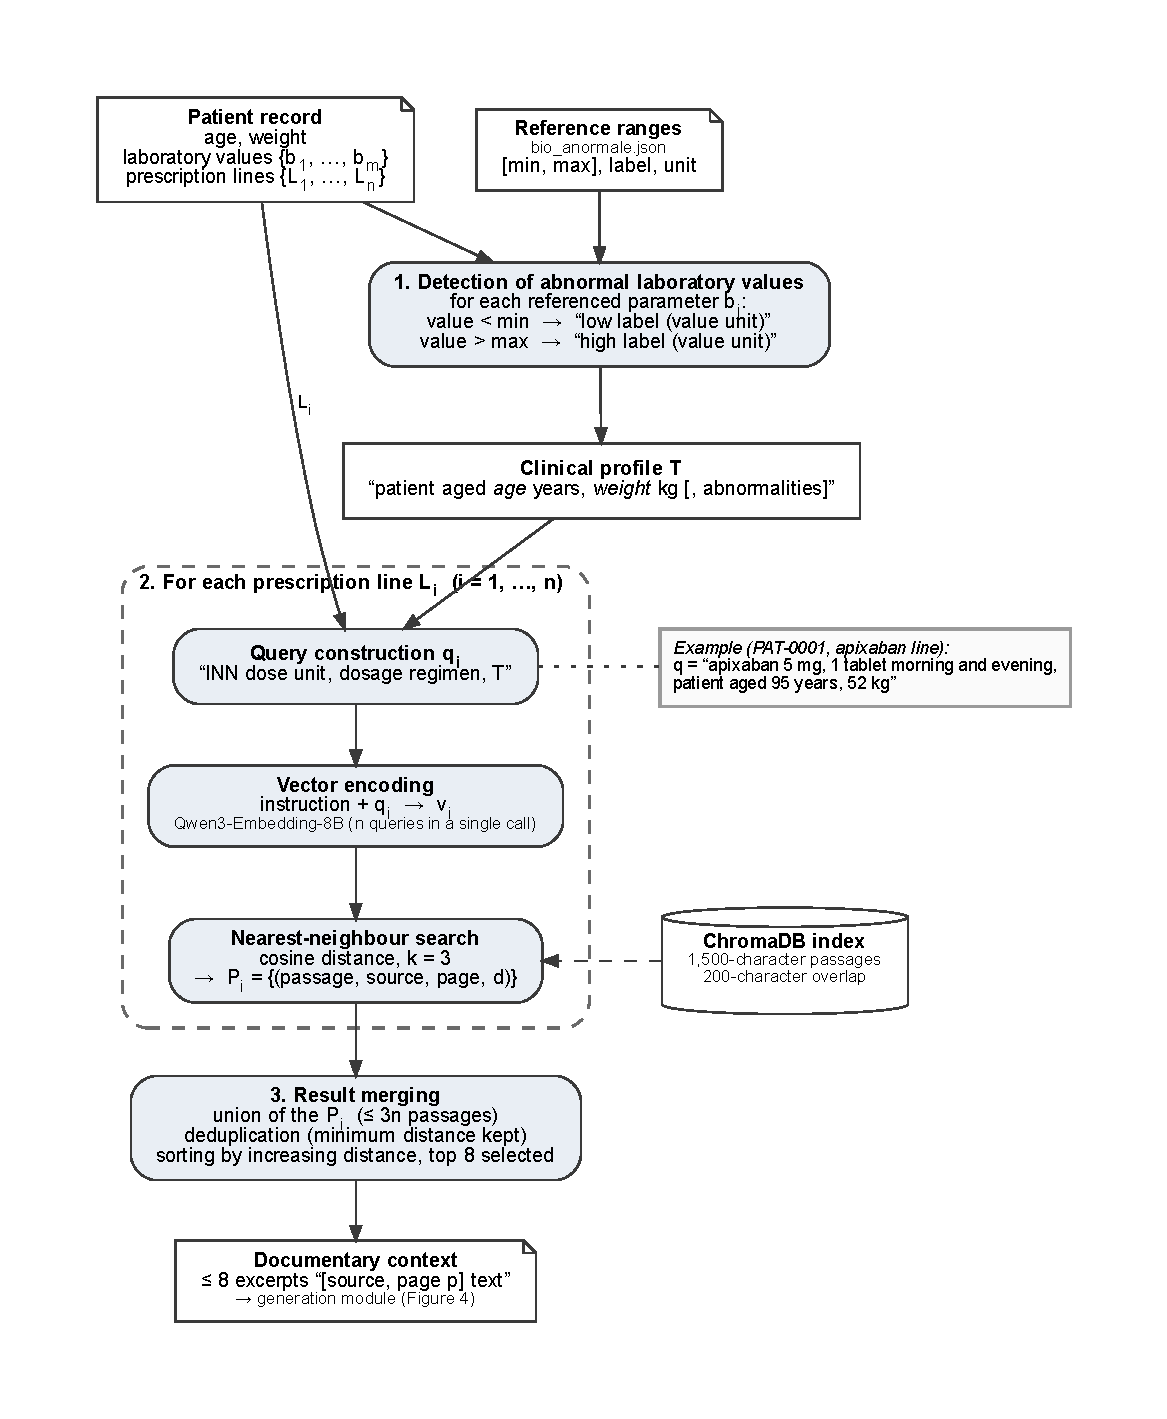
\includegraphics[width=0.75\textwidth]{figures_en/figure_2.pdf}
	\caption{Retrieval of relevant guideline passages for one patient. The renal values and the abnormal laboratory values are added to the clinical profile. One query is built for each prescription line, encoded with Qwen3-Embedding-8B and used for a 3-nearest-neighbour search (cosine distance). Retrieved passages are deduplicated and sorted by distance, and the eight closest are kept. The LLM then writes short context sentences about the patient, in French and in English. They are used as additional queries, and up to four new passages are added after the eight first ones. These passages form the context passed to the LLM.}
	\label{fig:retrieval}
\end{figure}

\subsection{Rule-based expert system}

The expert system applies deterministic rules to the patient record (Figure~\ref{fig:expert}). It is built on the CLIPS inference engine, used from Python with the clipspy library. The knowledge base is split into four files:
\begin{itemize}
	\item \texttt{base.clp}: the fact model, the unit conversions, the dose computations and the generic interaction rule;
	\item \texttt{generic\_rules.clp}: 1,877 drug interactions. Of these, 1,368 come from the Thesaurus of drug interactions of the French medicines agency (ANSM, September 2023) and 509 are pharmacokinetic interactions from DDI-Predictor, based on observed changes in the area under the curve (AUC). Each interaction is stored as a fact that gives two groups of drugs and the alert message;
	\item \texttt{personalized\_rules.clp}: hospital-specific rules, for example on the dose of apixaban or daptomycin;
	\item \texttt{statistical\_rules.clp}: situations in which the pharmacists of the hospital often make a pharmaceutical intervention. They were drawn from the 992 interventions written by the pharmacists in the prescription records. A situation was kept when at least 20 patients had an intervention on this theme, and when an intervention was made for at least 4\% of the treated patients. The file covers eight drug classes (oral anticoagulants, gout treatments, proton pump inhibitors, statins, levothyroxine, antidepressants, antidiabetic drugs and urological treatments) and a 25-OH vitamin D below 75~nmol/L.
\end{itemize}

\textbf{Translation into facts.} For each patient, the record is translated into CLIPS facts. Numeric data (age, weight, height, body mass index, body surface area and laboratory values) become \texttt{data} facts. Each prescription line becomes a \texttt{treatment} fact with its daily quantity and intake unit, and one \texttt{ingredient} fact for each active ingredient with its dosage. To identify the drugs, each label is converted to lowercase without accents. Every sequence of consecutive words of the label then becomes a \texttt{prescribed} fact. A rule can thus find ``apixaban'' in the label ``APIXABAN 5 MG (ELIQUIS), CPR'', whatever its position, and only whole words are matched.

\textbf{Inference.} The inference engine then runs in forward chaining. Some rules deduce new facts from the patient facts: the dose in mg per administration day, then the dose in mg/kg when the weight is known. These new facts can in turn trigger other rules. The generic interaction rule raises an alert when a drug of each group of an interaction is prescribed, on two distinct lines; a fixed-dose combination on a single line does not trigger it. This rule has a lower priority (salience), so that the alerts of the hospital rules are listed first. The statistical rules have the lowest priority, so their alerts are listed last. Their messages start with ``Patient à risque'' (at-risk patient): they report no problem, but point to the drugs that the pharmacists often need to review. A condition on a missing value is never satisfied. For example, the apixaban rule is made of four CLIPS rules. Three rules deduce the criteria (age $\geq$ 80 years, weight $\leq$ 60~kg, serum creatinine $\geq$ 133~$\mu$mol/L). The fourth raises an alert when the dose is not 2.5~mg and at least two criteria are met.

Each alert contains its message and the prescription lines involved. The output of the expert system is the list of alerts, with one alert per message. This list may be empty.

\begin{figure}[ht]
	\centering
	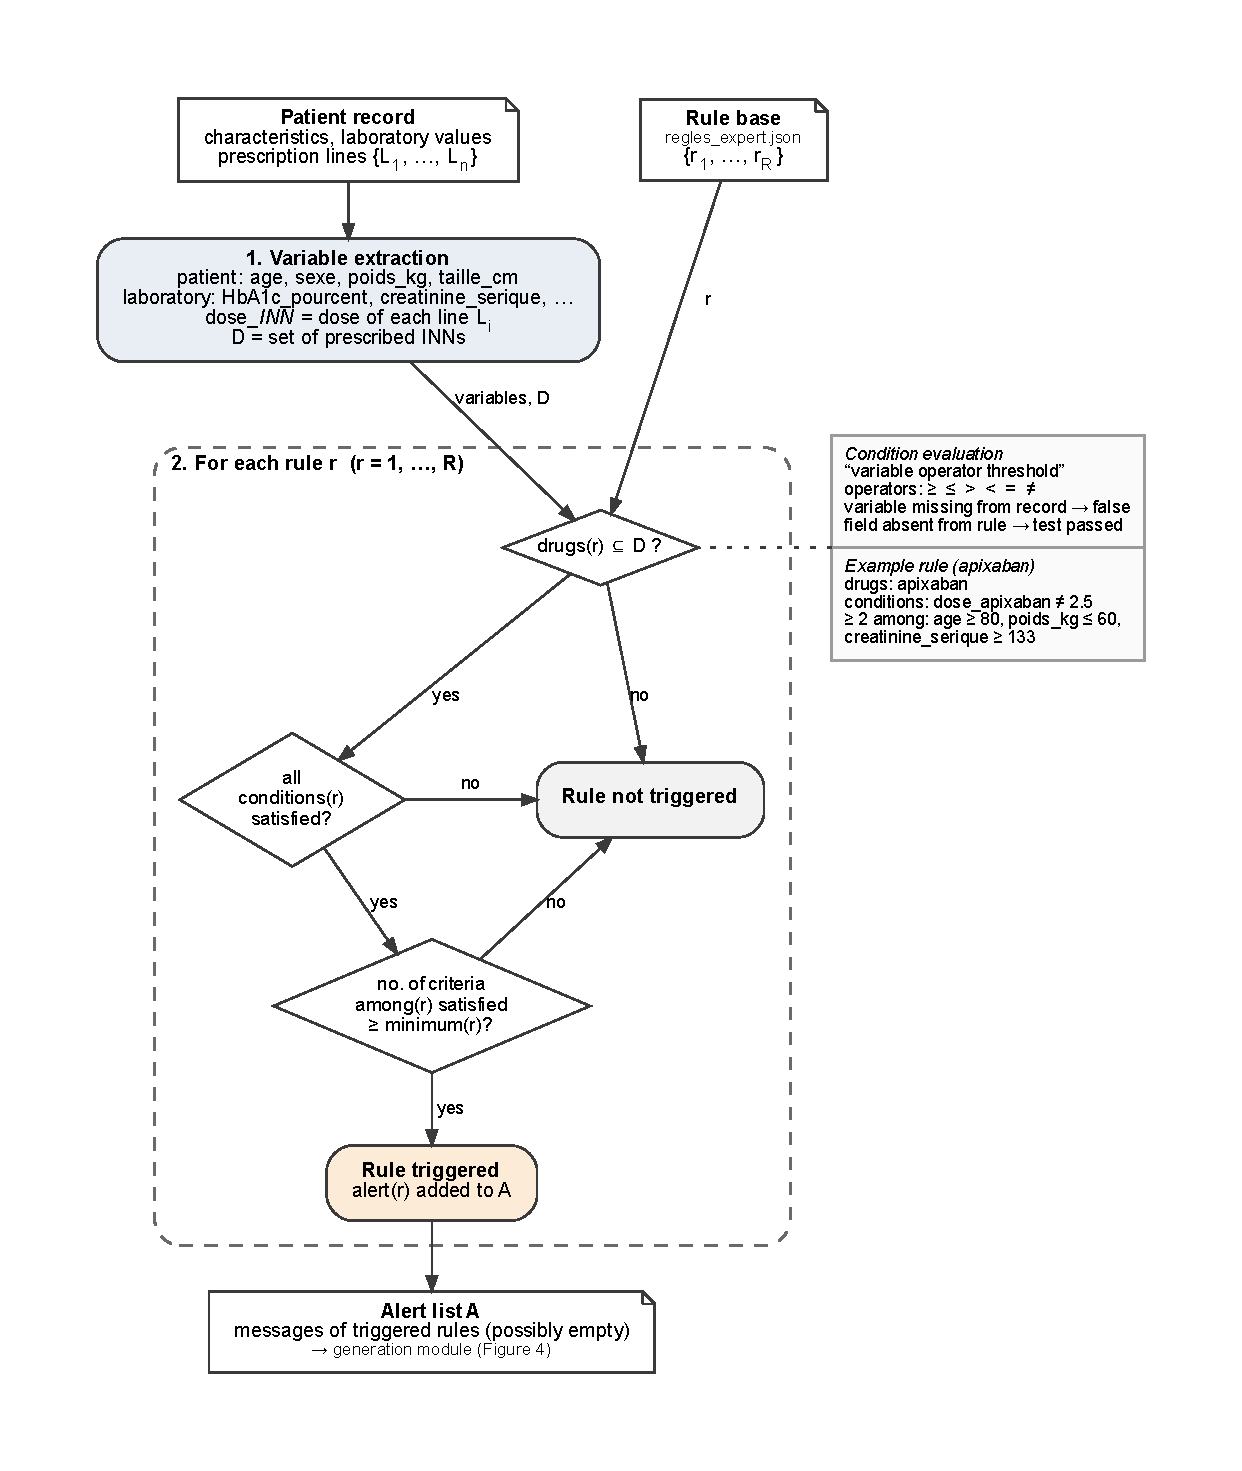
\includegraphics[width=0.75\textwidth]{figures_en/figure_3.pdf}
	\caption{Rule-based expert system (CLIPS). The patient record is translated into facts and loaded, with the knowledge base, into the working memory. The inference engine fires the rules whose patterns are matched, in forward chaining: deduced facts, such as the dose per kg, can trigger other rules. The alert facts form the list of alerts passed to the LLM. New hospital rules are drafted by the LLM from a pharmacist request (create\_rule.py) and saved in the knowledge base.}
	\label{fig:expert}
\end{figure}

\subsection{Drafting of new rules with the LLM}

Pharmacists do not need to write CLIPS code to add a hospital rule. They write a request in natural language, for example ``Alert if metformin is prescribed with an eGFR below 30~mL/min''. The LLM translates this request into CLIPS code. Its prompt describes the available facts, the exact names and units of the laboratory parameters found in the patient records, and two example rules. The model is the same as for the pharmaceutical opinion, with a temperature of 0, the reasoning mode disabled and a JSON output.

The proposed rule is then checked automatically. It must contain at least one rule, must not use CLIPS functions that access files or the system (such as \texttt{system}, \texttt{open} or \texttt{eval}), must not reuse the name of a rule of the base file, and must load without error in CLIPS. The interface shows the rule, its alert messages and the number of patient records for which it would be triggered. The rule is added to \texttt{personalized\_rules.clp} only when the pharmacist confirms it. Saved rules can also be deleted from the interface.

\subsection{Generation of the pharmaceutical opinion}

The final decision is made by an LLM (Figure~\ref{fig:generation}). We used Qwen3.6-35B-A3B, accessed through the OpenRouter API. The temperature was set to 0. The reasoning mode was enabled: in our tests, it gave much more consistent opinions, but the analysis took about 40~s per patient instead of 10~s. The output was limited to 12,000 tokens, and the model was required to answer in JSON format.

\textbf{User message.} The patient record is summarized before it is sent to the model. Empty fields are removed. Each laboratory value is given with its unit and date, and is marked ``low'' or ``high'' when it is outside the reference range. Each prescription line receives an identifier (L1, L2, \ldots) and a status on the reference date (ongoing, ended or upcoming). When it can be computed, the dose of active ingredient per administration day is added, so that the model does not have to compute it. When the same drug is prescribed on several ongoing scheduled lines, these lines are listed with their total dose. The message then contains the expert system alerts, labelled A1, A2, \ldots, and the retrieved passages, labelled R1, R2, \ldots, with their file and page.

\textbf{System prompt.} The model acts as a French hospital clinical pharmacist and answers in English. The prompt states that the record contains no diagnosis, medical history or indication. The model must therefore not judge the indication of a drug, and each point must rely on a fact of the record, an alert or a passage. When a point relies only on the knowledge of the model, an intervention or a verification may only be proposed for an obvious error, such as a dose above the maximum dose or a contraindication confirmed by the laboratory values. The prompt also explains the four levels of the ANSM Thesaurus: contraindication, combination not recommended, precaution for use and ``to be taken into account''. Contraindications take priority. The other alerts justify an intervention only if the risk is clinically critical for this patient, so an alert never justifies an intervention on its own. The alerts of the statistical rules report no problem: the model must examine the drugs involved more carefully, but must never make a point only because of such an alert. Finally, the model must check that each point is consistent with the patient: the exceptions written in the alerts, the direction of laboratory abnormalities (a treatment that corrects an abnormal value is justified by this value) and the dates of the lines.

\textbf{Output.} The model first returns a short reasoning of three to six sentences. It then returns one to four points, from the most to the least important. Each point has one of four types:
\begin{itemize}
	\item \texttt{intervention}: a confirmed and clinically important problem requires a change in the prescription;
	\item \texttt{verification}: information missing from the record is needed to decide, and the problem would justify an intervention if it were confirmed (for example, the same drug on several lines);
	\item \texttt{monitoring}: the prescription is acceptable but justifies a specific clinical or laboratory monitoring;
	\item \texttt{validation}: nothing to report.
\end{itemize}
Each point is a short proposal of at most 40 words. It gives the identifiers of the alerts and passages it relies on and, for an intervention, the identifiers of the lines to modify.

\textbf{Post-processing.} The answer is parsed as JSON. The identifiers cited by the model are replaced by the corresponding alerts, documents and prescription lines. Unknown identifiers are ignored, so the model cannot cite a source that was not provided. A validation point is removed when another point is present. The decision for the patient is the type of the most severe point: pharmaceutical intervention proposed, verification proposed, monitoring proposed or patient validated. If the analysis fails, the error is saved and the record can be analysed again.

\begin{figure}[ht]
	\centering
	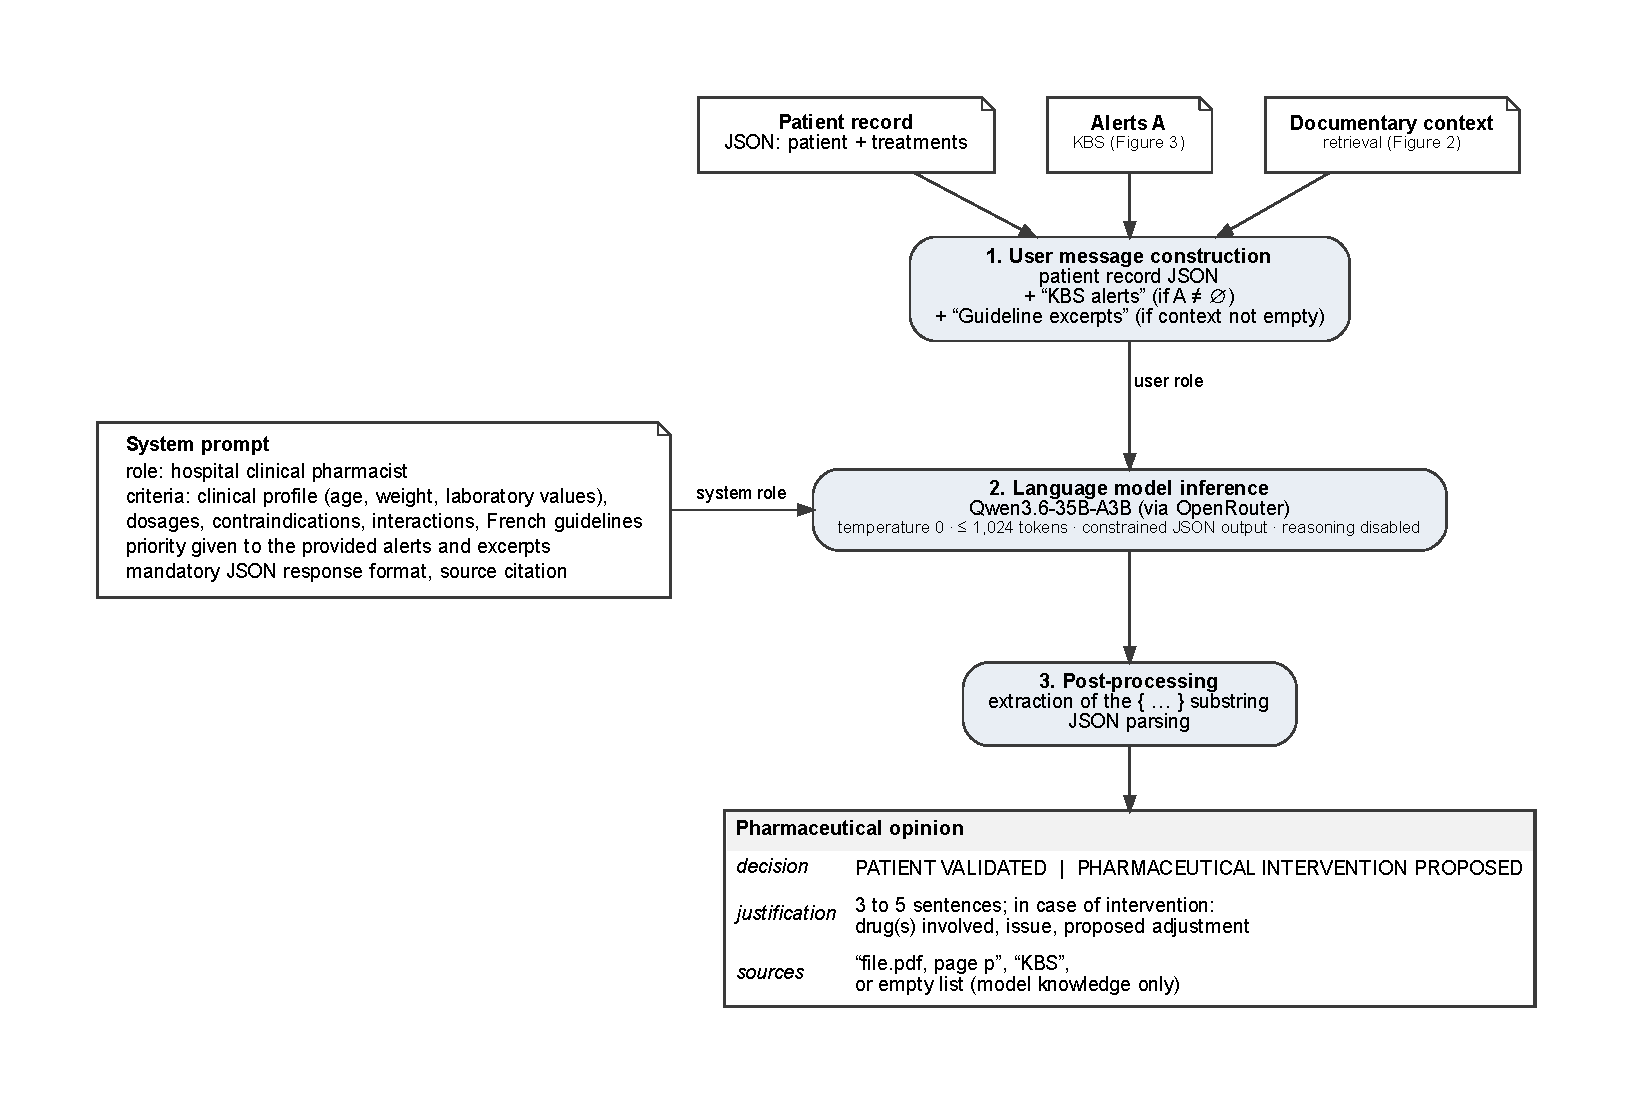
\includegraphics[width=0.85\textwidth]{figures_en/figure_4.pdf}
	\caption{Generation of the pharmaceutical opinion. The user message combines a summary of the patient record, the expert system alerts and the retrieved guideline passages, each with an identifier. The system prompt defines the role of the model, the limits of the record and the use of the alerts. The model (Qwen3.6-35B-A3B, temperature 0, reasoning enabled, JSON output) returns a short reasoning and one to four typed points. The cited identifiers are replaced by the alerts, documents and lines, and the decision is the most severe point.}
	\label{fig:generation}
\end{figure}

\subsection{Implementation}

The pipeline was written in Python. A graphical interface was built with Streamlit for use by pharmacists. It allows users to run the analysis of the records that have not been analysed yet, to read the results, and to open the cited sources at the relevant page. It also allows users to add new guidelines to the document base, and to add expert system rules drafted by the LLM or to delete them. These changes do not require any programming. Finally, the pharmacist can score each opinion from 0 (error or not relevant) to 5 (very relevant). The scores are saved with the patient identifier.

% TODO: Evaluation (dataset, reference standard, metrics)


\section{Results}
\label{sec:results}

% TODO: Performance results

\subsection{Graphical interface}

Figure~\ref{fig:interface_list} shows the main screen of the interface. The top of the screen gives the number of records and of analysed records, the number of records for each decision (interventions, verifications, monitoring and validations), and the number of errors and of records not yet analysed. Records can be filtered by status and searched by patient identifier or drug name. Records that need an action are shown first.

For each patient, the interface shows the patient profile, the laboratory values, the prescription, the decision and the points of the opinion, each with its sources (Figure~\ref{fig:interface_patient}). Abnormal laboratory values and the prescription lines that the model proposes to modify are shown in red. Each expert system alert can be opened to read its level, its message and the recommended action (Figure~\ref{fig:interface_alert}).

Each cited source can be opened with one click. The PDF is then shown at the page cited by the model (Figure~\ref{fig:interface_source}). This allows the pharmacist to check quickly the information used by the model.

A second page shows the hospital rules of the expert system (Figure~\ref{fig:interface_rules}). The pharmacist writes a request in natural language to draft a new rule. Each saved rule is shown with its alert message and the conditions that trigger it, and can be deleted. A third page lists the indexed guidelines with their number of passages (Figure~\ref{fig:interface_documents}). New PDF documents can be uploaded and indexed from this page.

\begin{figure}[ht]
	\centering
	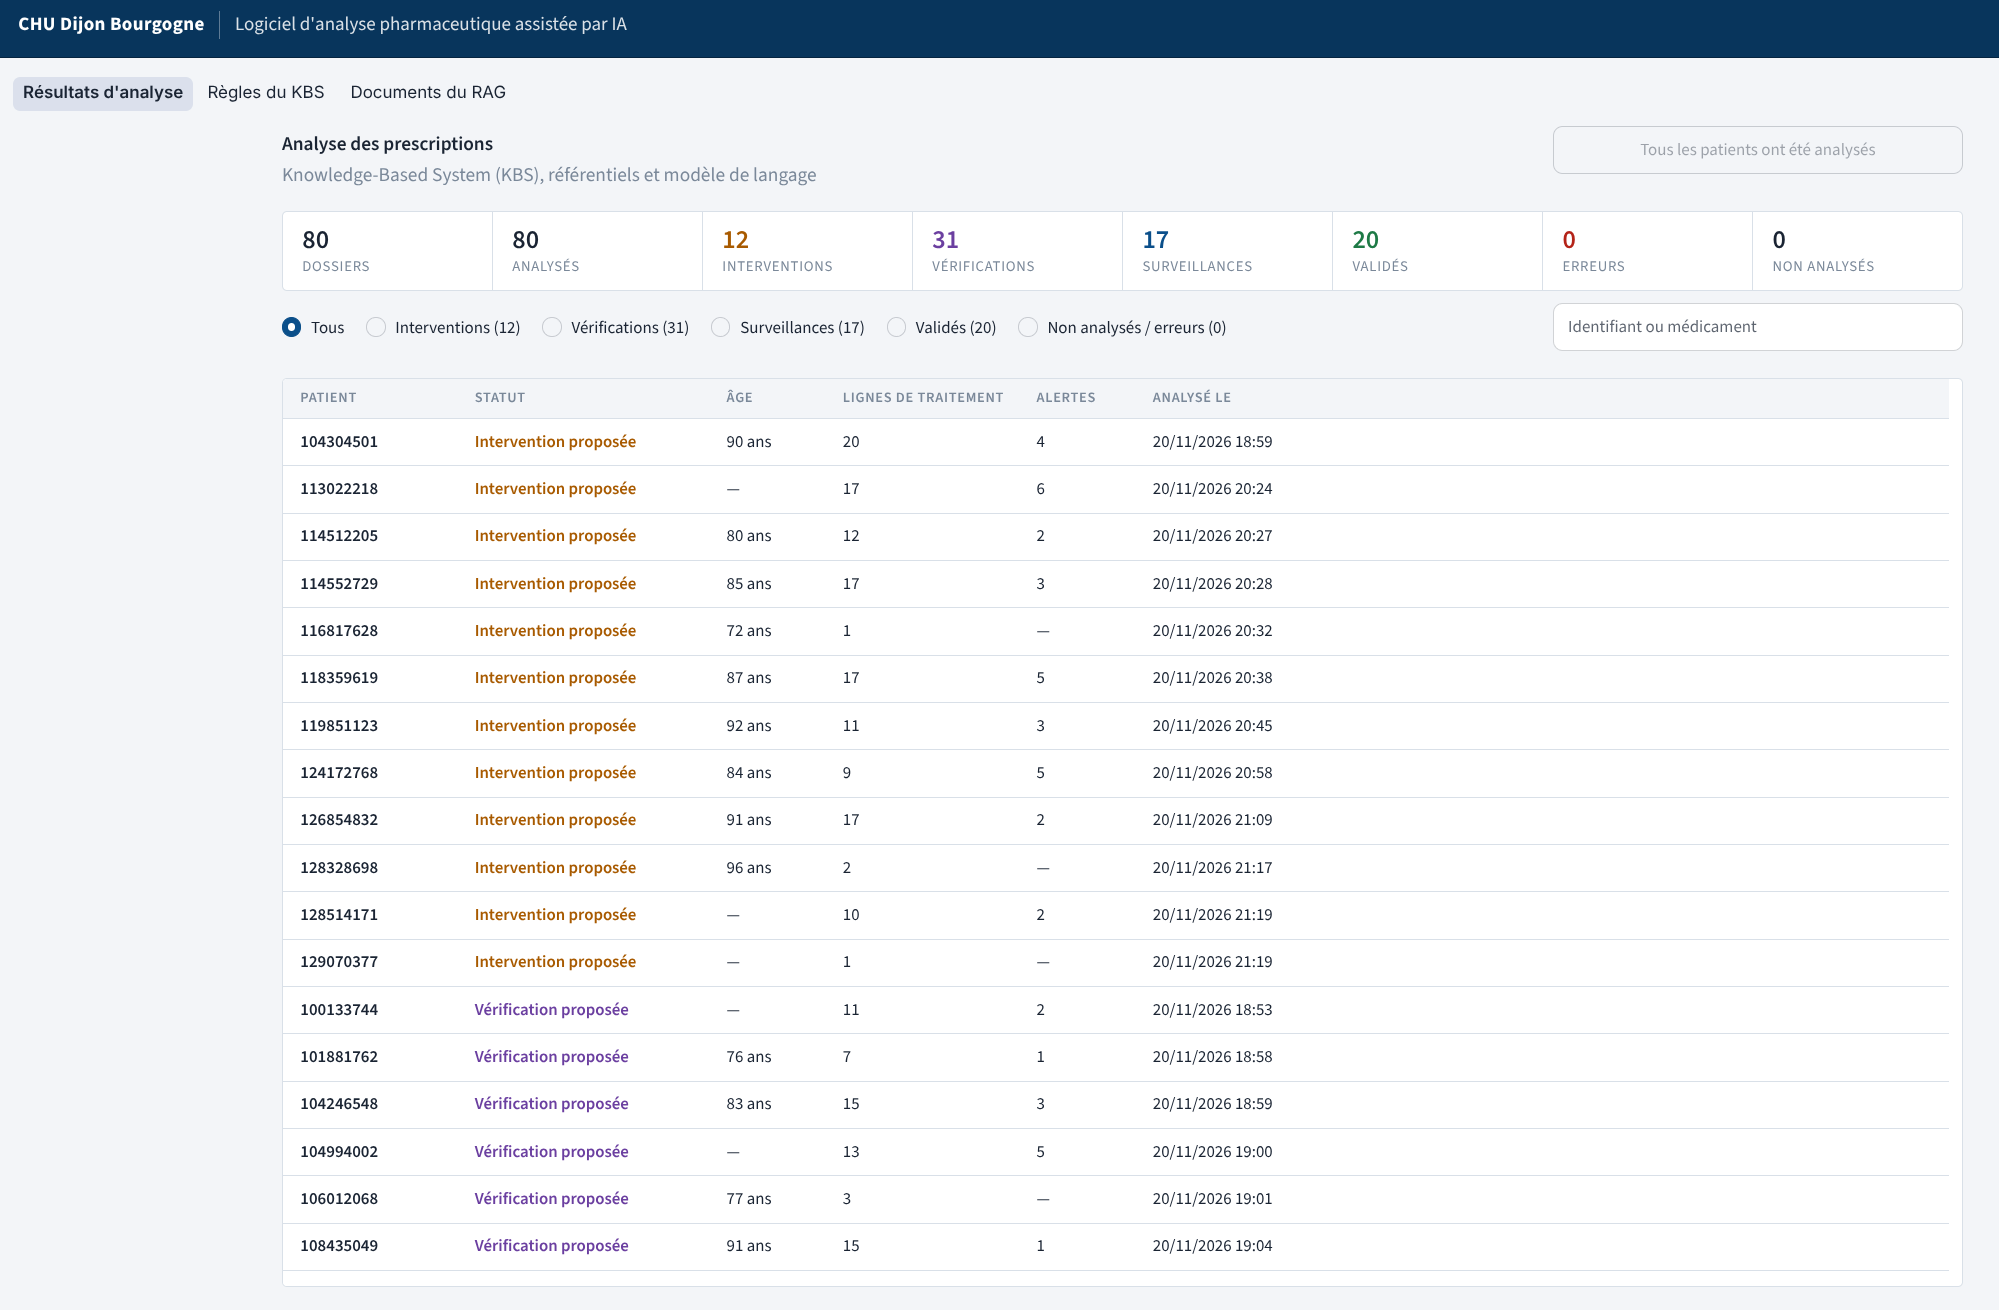
\includegraphics[width=\textwidth]{screenshots/screenshot1.png}
	\caption{Main screen of the graphical interface. The top of the screen gives the number of records for each decision. The records can be filtered by decision and searched by patient identifier or drug name.}
	\label{fig:interface_list}
\end{figure}

\begin{figure}[ht]
	\centering
	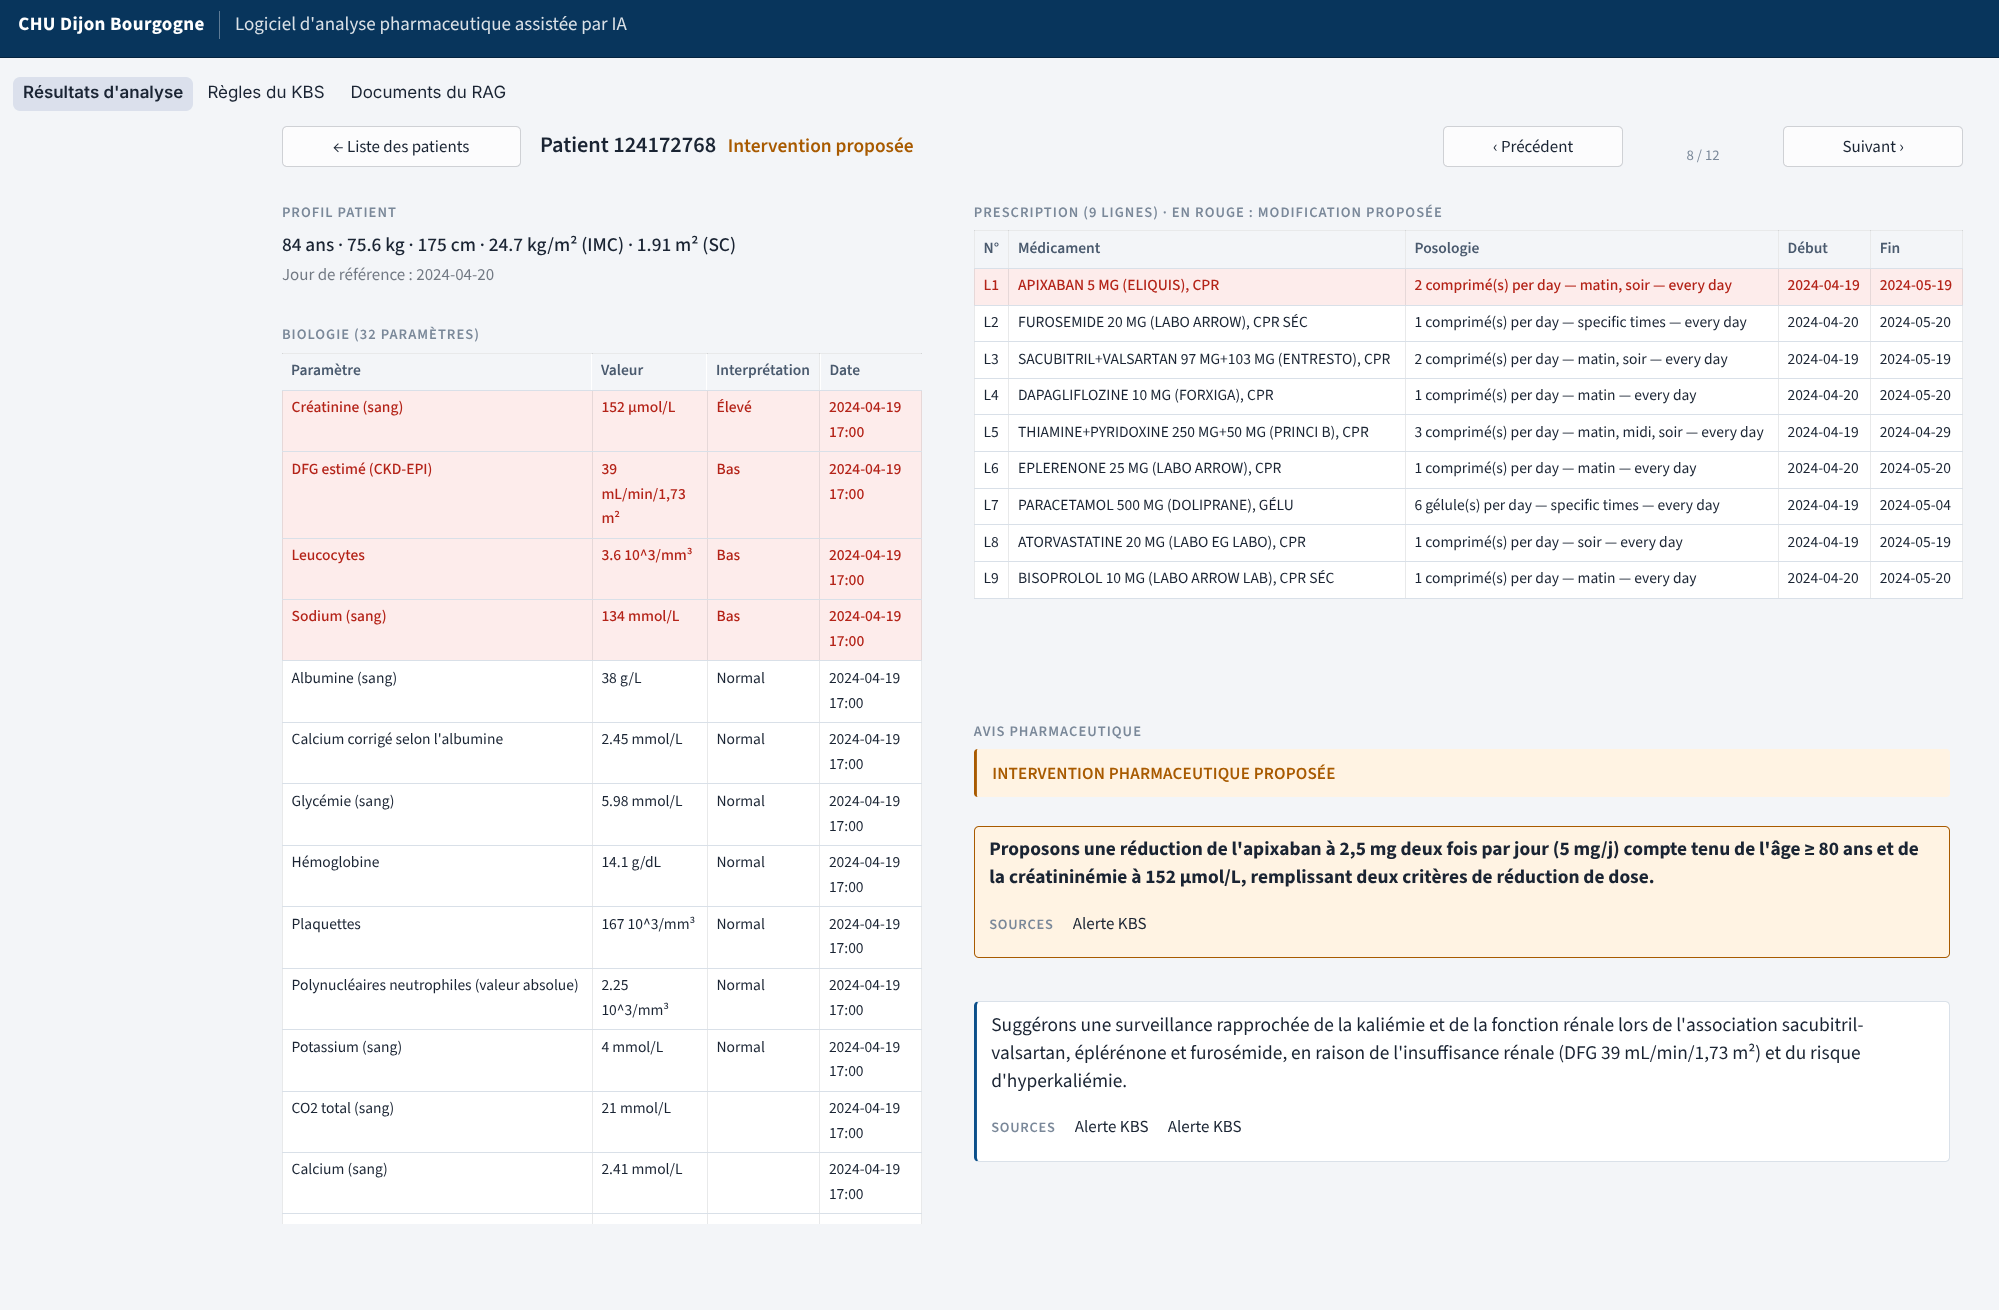
\includegraphics[width=\textwidth]{screenshots/screenshot2.png}
	\caption{Record of one patient. The interface shows the patient profile, the laboratory values, the prescription and the pharmaceutical opinion with its sources. Abnormal laboratory values and the line to modify are shown in red.}
	\label{fig:interface_patient}
\end{figure}

\begin{figure}[ht]
	\centering
	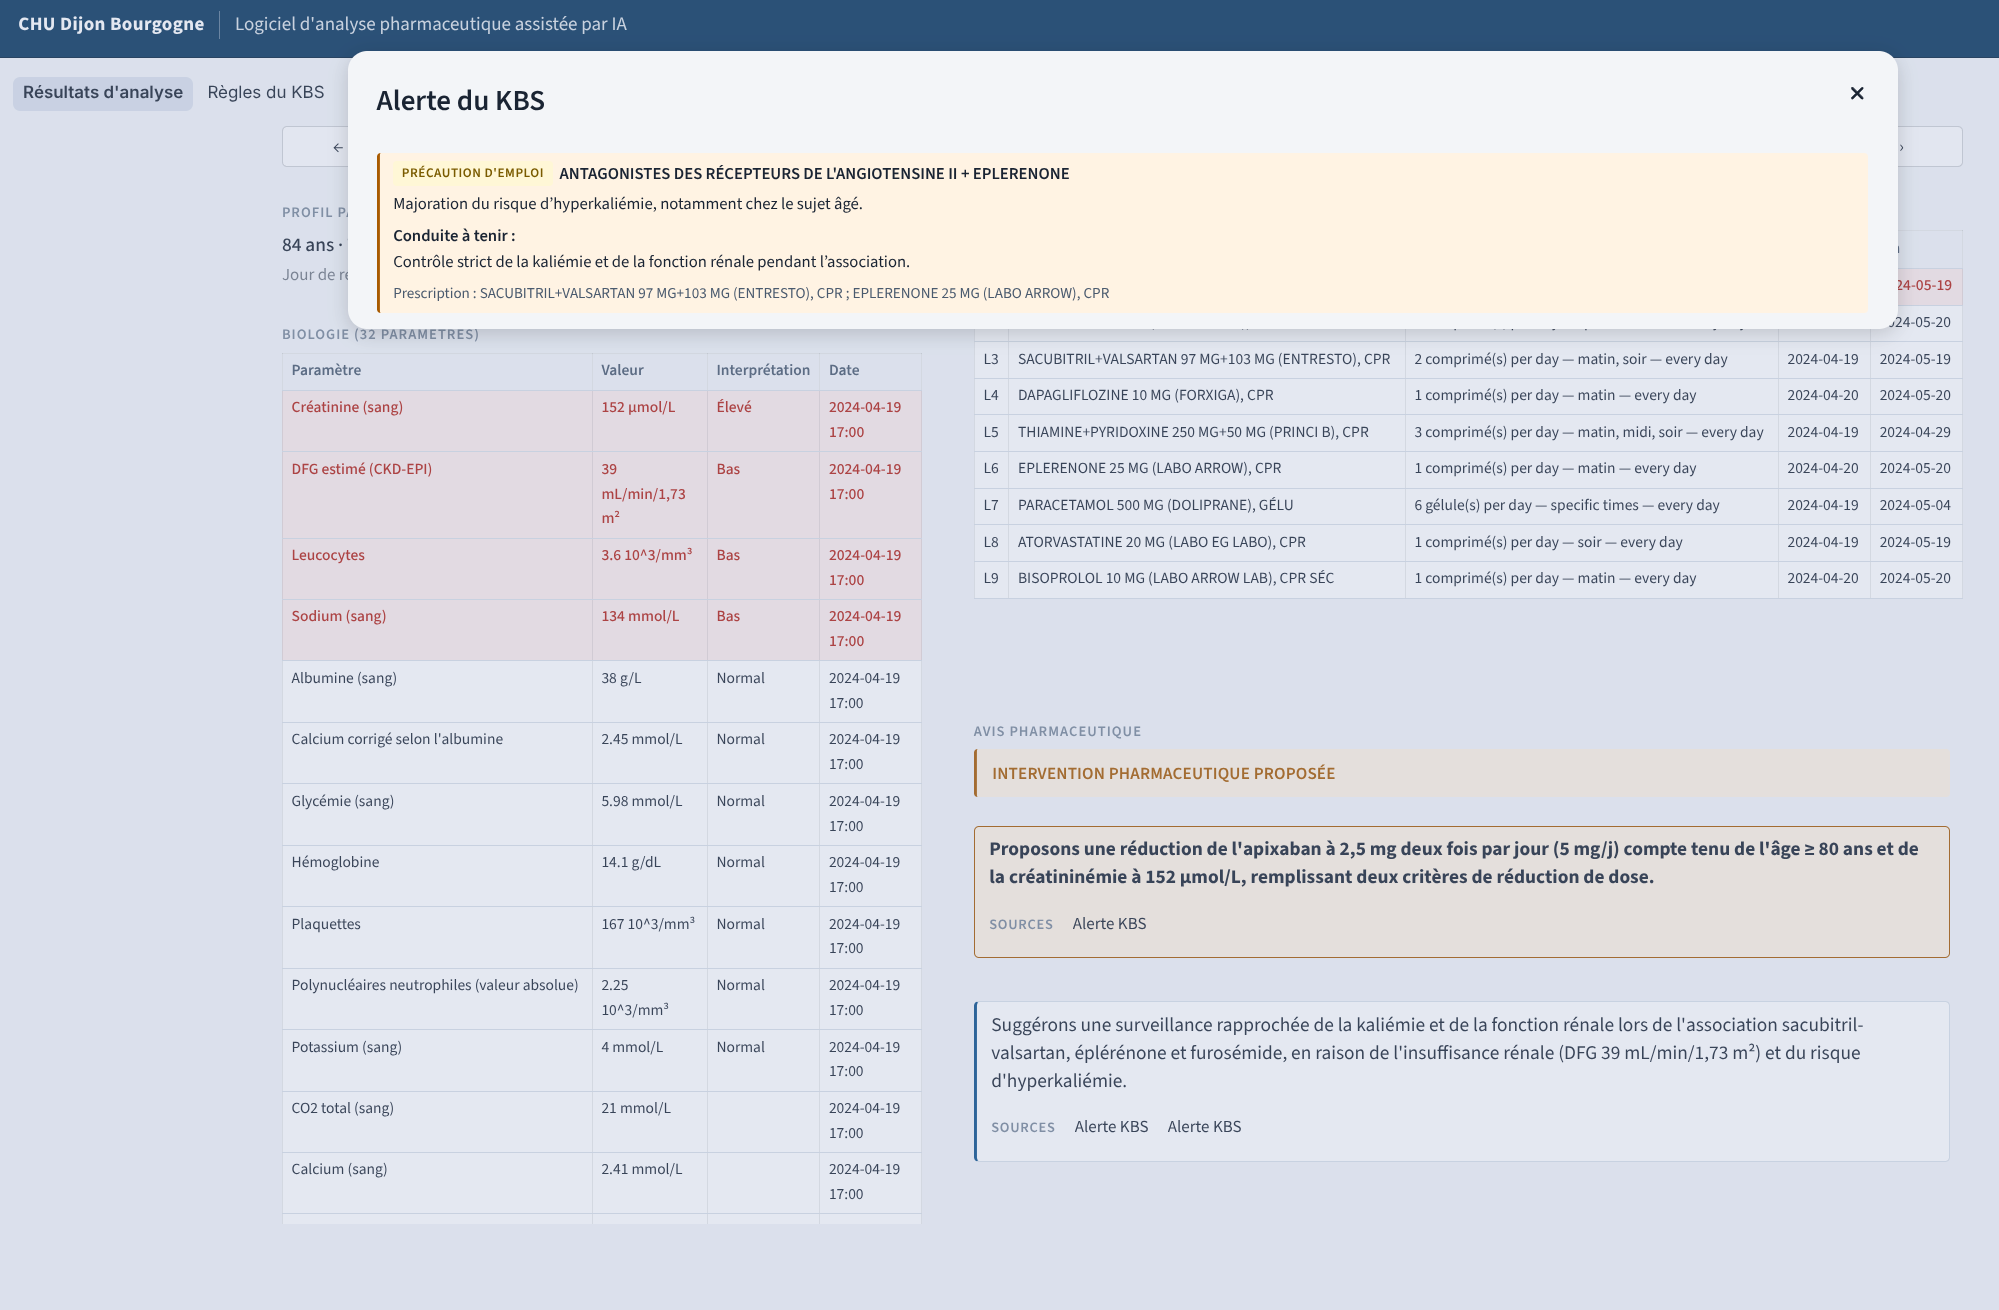
\includegraphics[width=\textwidth]{screenshots/screenshot6.png}
	\caption{Display of an expert system alert. The alert gives its level, its message, the recommended action and the prescription lines involved.}
	\label{fig:interface_alert}
\end{figure}

\begin{figure}[ht]
	\centering
	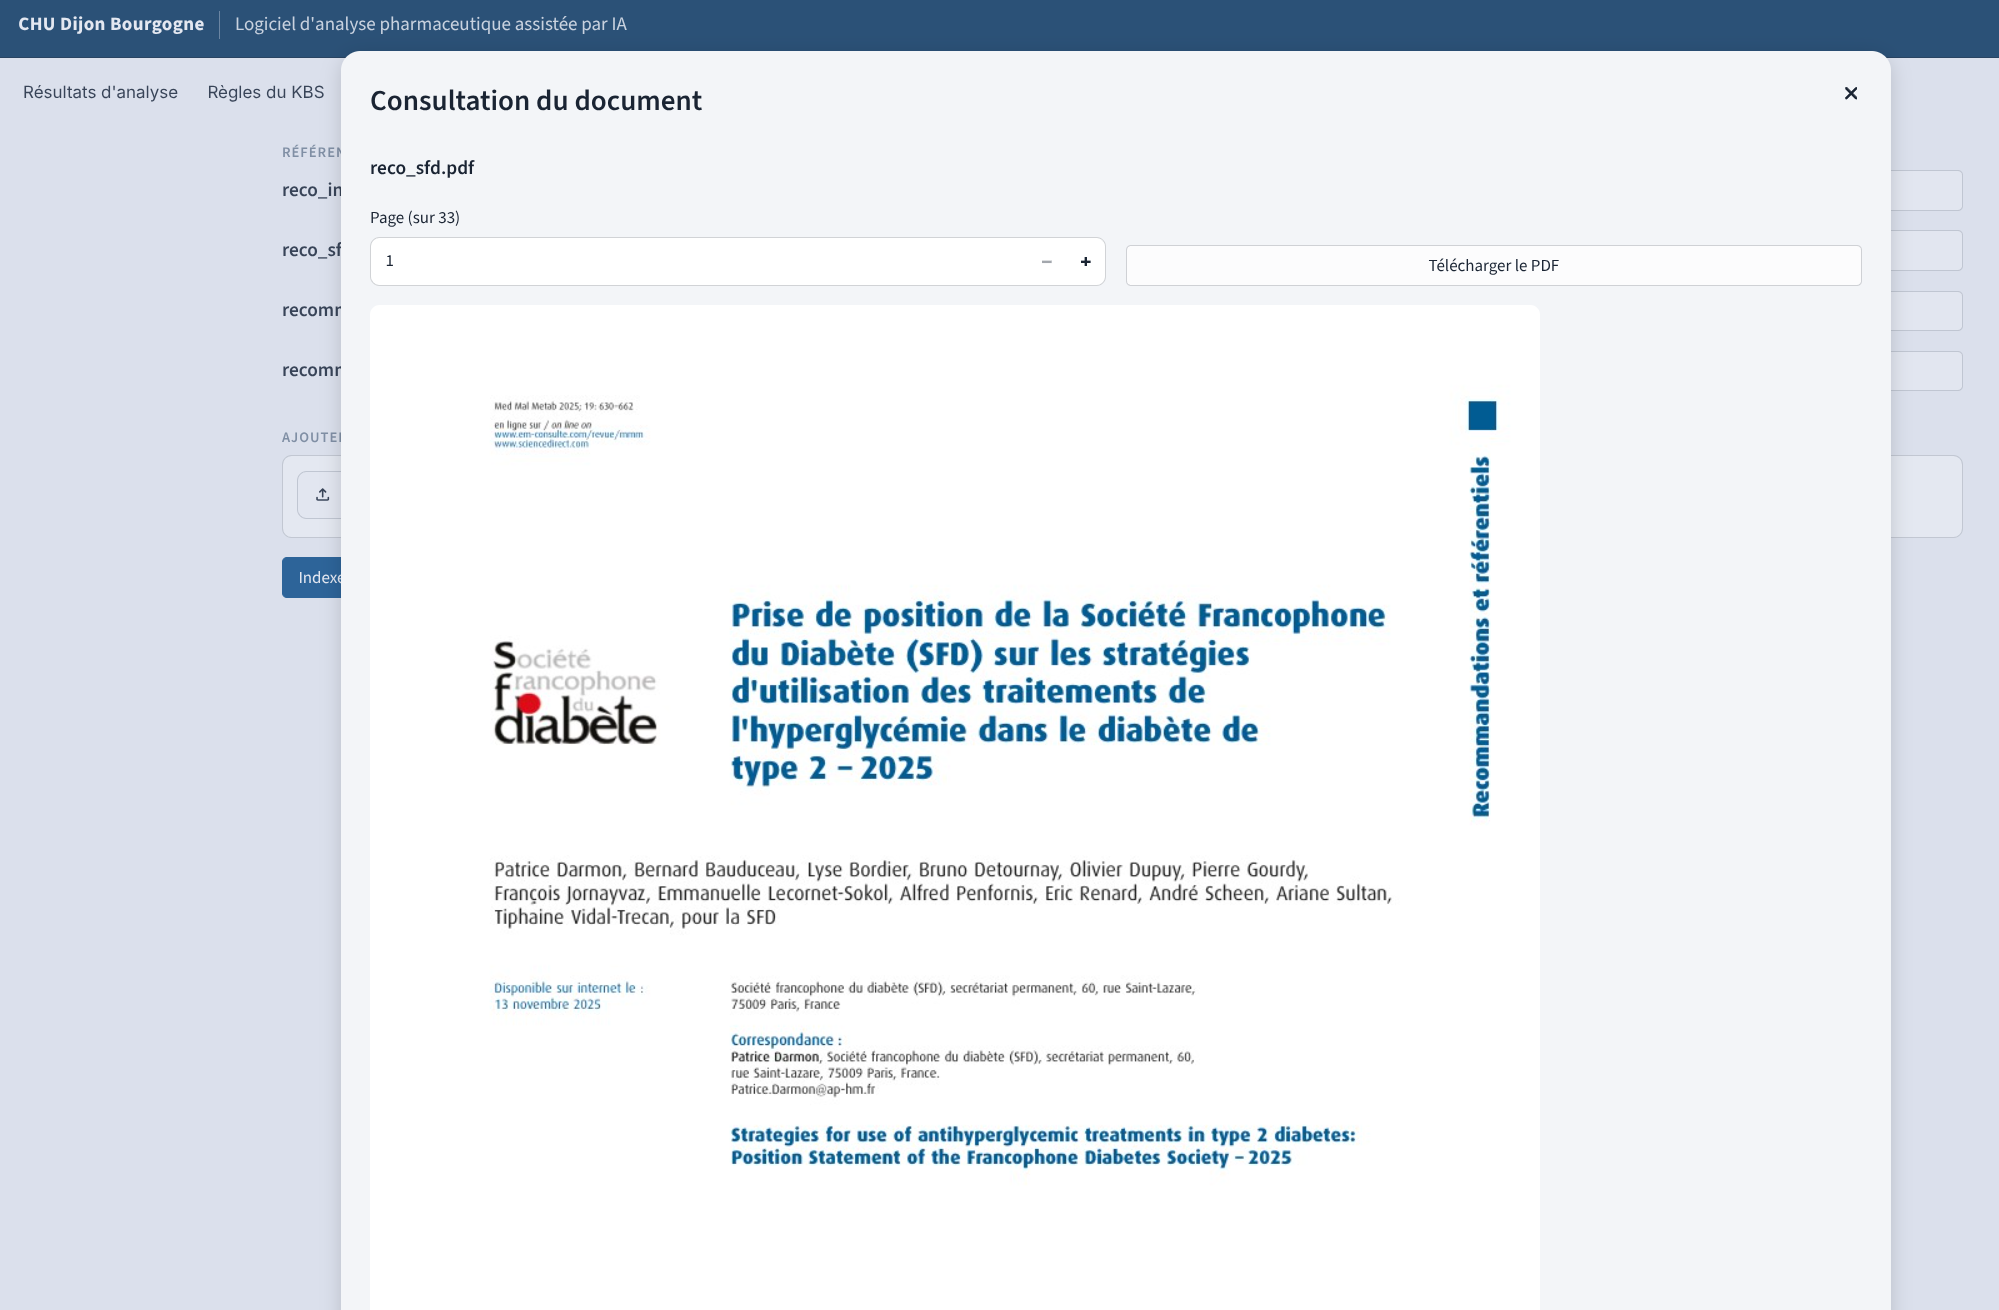
\includegraphics[width=\textwidth]{screenshots/screenshot5.png}
	\caption{Display of a guideline document. Clicking on a reference opens the document at the page cited by the model.}
	\label{fig:interface_source}
\end{figure}

\begin{figure}[ht]
	\centering
	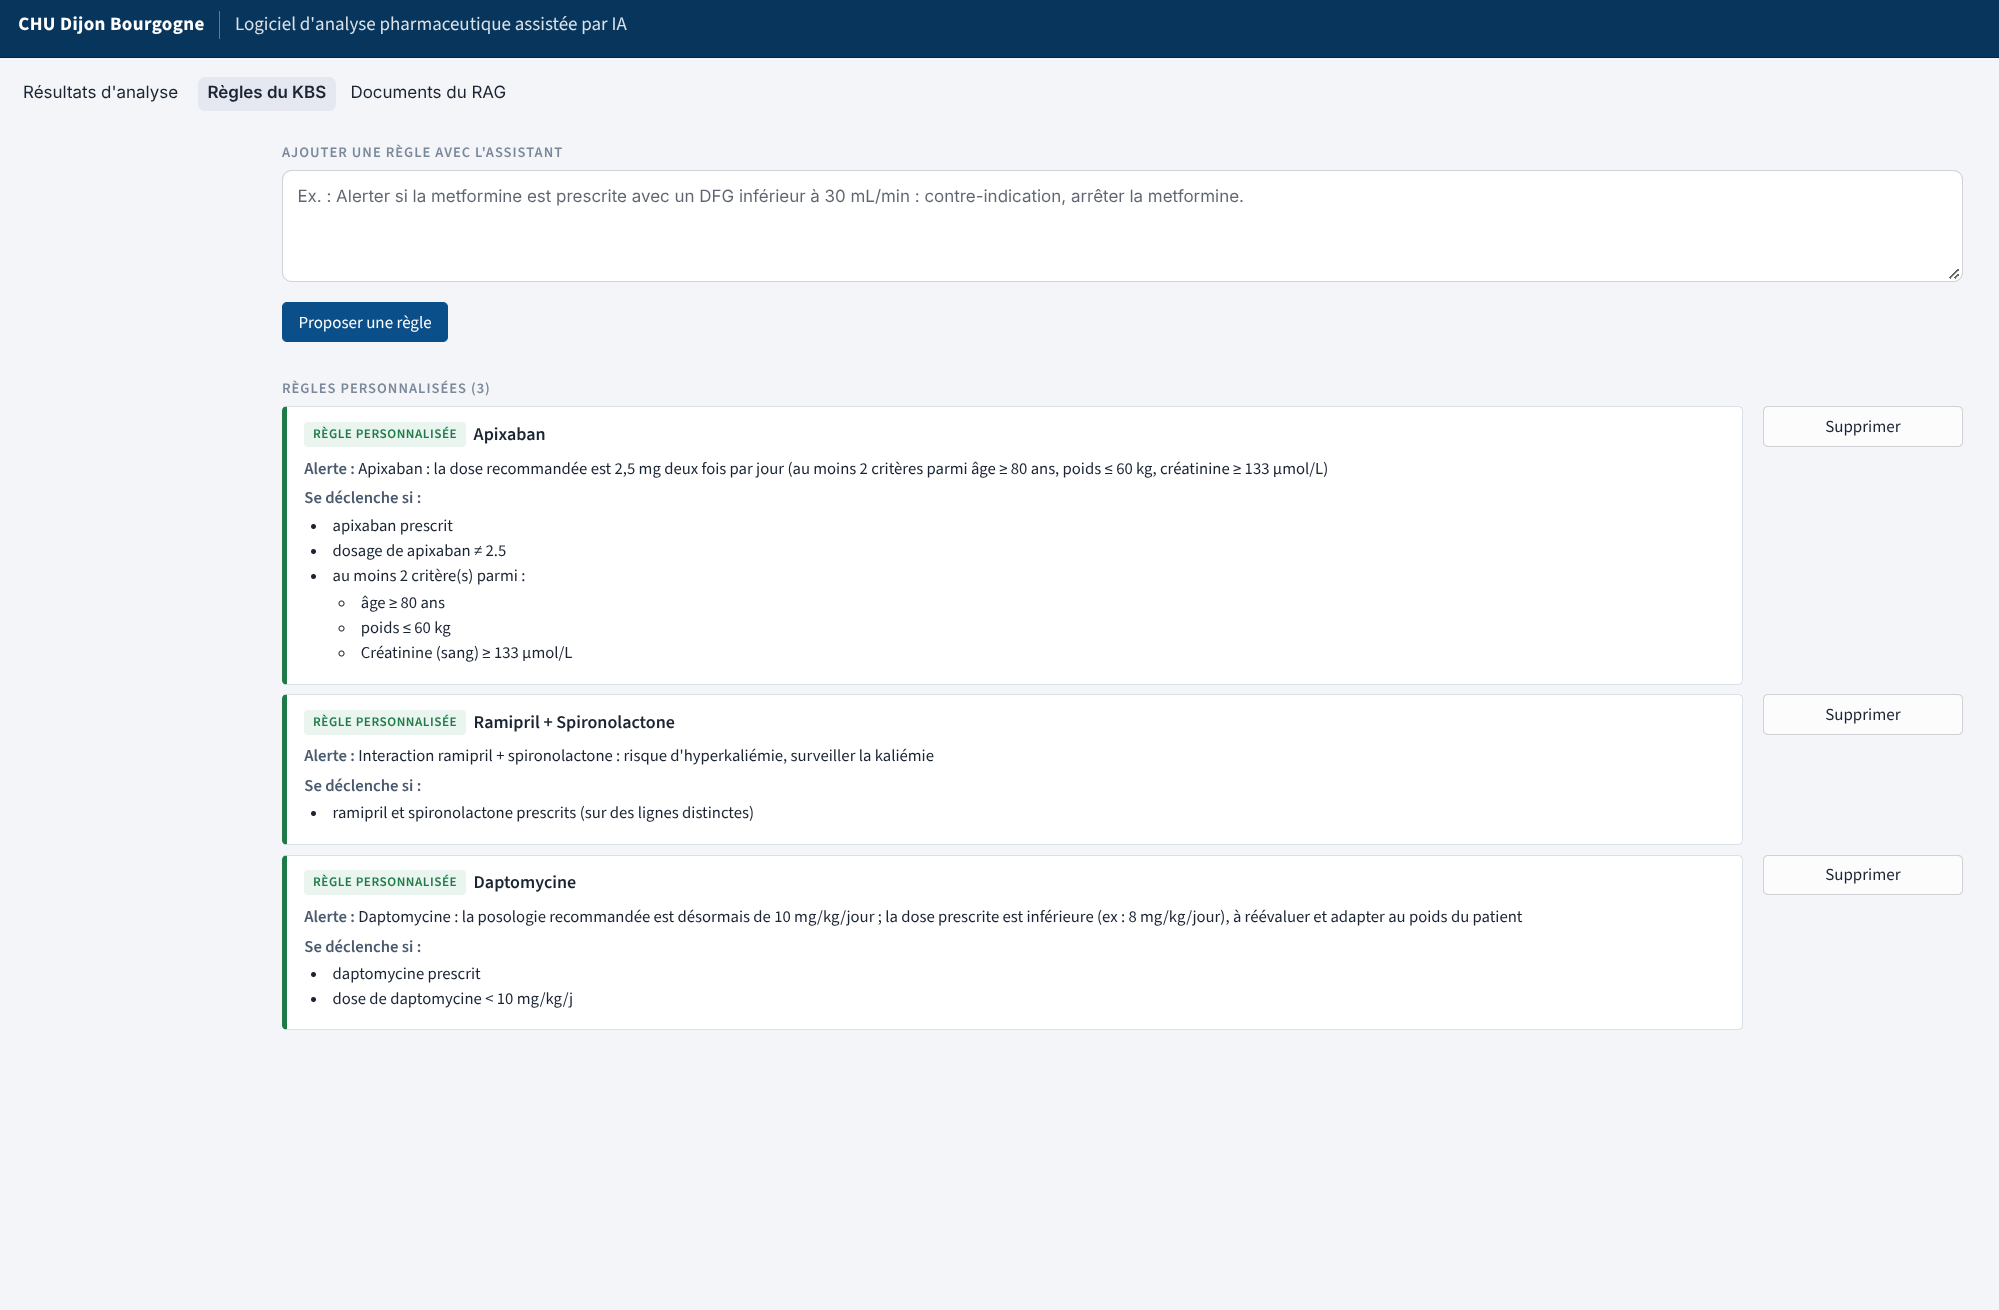
\includegraphics[width=\textwidth]{screenshots/screenshot3.png}
	\caption{Page of the expert system rules. A new rule is drafted by the LLM from a request in natural language. Each saved rule is shown with its alert message and the conditions that trigger it.}
	\label{fig:interface_rules}
\end{figure}

\begin{figure}[ht]
	\centering
	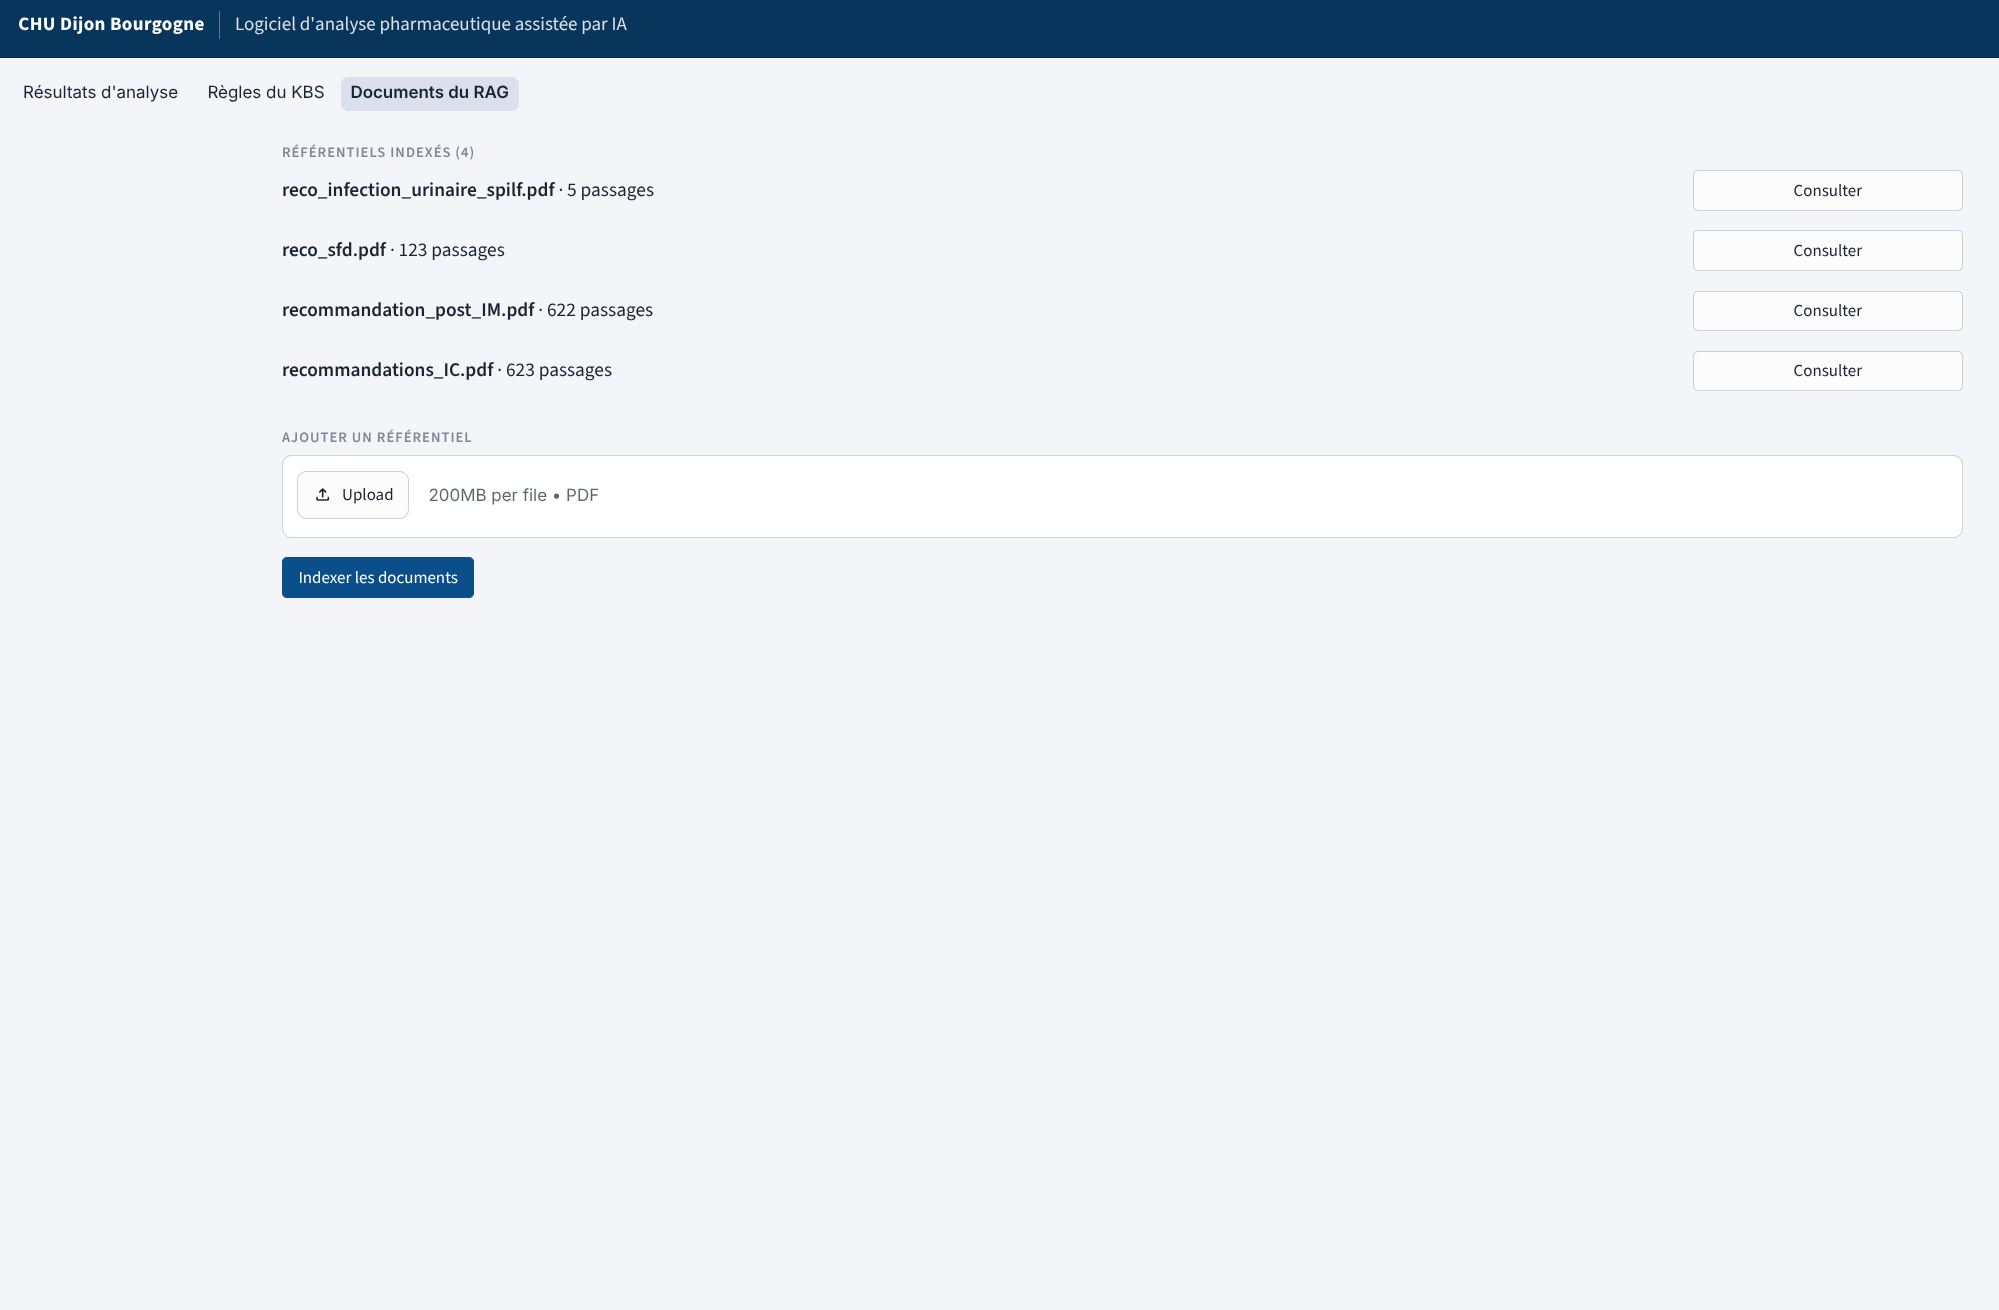
\includegraphics[width=\textwidth]{screenshots/screenshot4.png}
	\caption{Page of the guideline documents. The page lists the indexed documents with their number of passages, and allows users to add and index new PDF documents.}
	\label{fig:interface_documents}
\end{figure}


\section{Discussion}
\section{conclusion}
% TODO: Conclusion

% \bibliographystyle{unsrtnat}
% \bibliography{references}

\end{document}
